\scanpage{16}
$\deleted{\unsure{R|\beta}}$

\diagram{$\begin{array}{c|c|c|c|c|}
(u,v)&v=u&v=u'&\{u,v\}\in A_\alpha\deleted{\unsure{'}}&\{u,v\}\in A'_\alpha\\\hline
\det(u-v)&0&1&\alpha'&\alpha\\\hline
\operatorname{Tr}uv&1&0&\alpha&\alpha'\\\hline
\end{array}$}

\figure{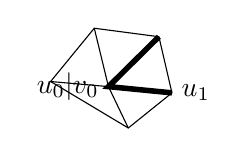
\begin{tikzpicture}[scale=.72]
\coordinate (a) at (0,.7);\coordinate (b) at (.77,1.64);\coordinate (c) at (1.91,1.49);\coordinate (d) at (2.14,.5);\coordinate (e) at (1.37,-.12);\coordinate (o) at (1.02,.61);
\draw (a)--(b)--(c)--(d)--(e)--cycle;
\draw (a)--(o)--(e) (b)--(o);\draw[line width=2pt] (c)--(o)--(d);
\node[left] at (o){$\unsure{u_0|v_0}$};\node[right] at (d){$u_1$};
\end{tikzpicture}}

\uline{Prop} Soient $u,v\in S_\alpha$, avec $v\ne u,u'$ Alors

\[
\begin{aligned}
\operatorname{Tr}v\,u^i(v)&=\alpha &&\text{si }i\deleted{\unsure{\ne}}\equiv1\text{ ou }-1\quad(5)\\
\operatorname{Tr}v\,u^i(v)&=\alpha' &&\text{si }\unsure{i'|i}\equiv2\text{ ou }-2\quad(5)\\
(&=1&&\text{si }i\equiv0\quad(5))
\end{aligned}
\]

\[
\begin{aligned}
\operatorname{Tr}uv_0&=1+\alpha(\lambda+\lambda^{-1})=1+\alpha=\alpha' &u^5&=\alpha\\
\unsure{T|\operatorname{Tr}}u\,v'_0&=\alpha
\end{aligned}
\]

\[
uv=\begin{pmatrix}1&0\\\alpha'&\alpha'\end{pmatrix}\qquad
u^{-1}v=\begin{pmatrix}0&1\\1&\alpha^{\unsure{2|{}|'}}\end{pmatrix}
\]

\[
\begin{aligned}
u_{\unsure{*|{}}}&=\begin{pmatrix}0&1\\\alpha&1\end{pmatrix}
&u^{-1}&=\begin{pmatrix}\alpha'&\alpha'\\1&0\end{pmatrix}\\
v_0&=\begin{pmatrix}1&\alpha\\1&0\end{pmatrix}\\
v_1&=uvu^{-1}=\begin{pmatrix}\alpha'&\alpha'\\1&\alpha^{\unsure{'|2|{}}}\end{pmatrix}\\
v_{-1}&=u^{-1}vu=\begin{pmatrix}\alpha&1\\\alpha^{\unsure{''|'}}&\alpha'\end{pmatrix}
\end{aligned}
\]

\figure{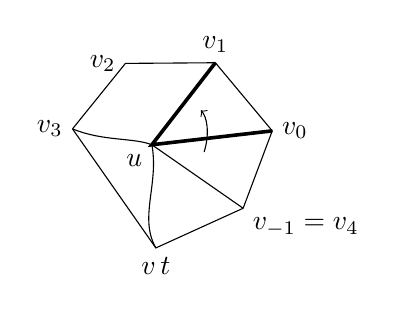
\begin{tikzpicture}[scale=.84]
\coordinate (a) at (-1.22,.1);\coordinate (b) at (-.42,1.09);\coordinate (c) at (.94,1.1);\coordinate (d) at (1.8,.07);\coordinate (e) at (1.36,-1.1);\coordinate (f) at (.04,-1.7);\coordinate (o) at (-.02,-.14);
\draw (a)--(b)--(c)--(d)--(e)--(f)--(a);
\draw (a)..controls(-.76,-.09)and(-.3,-.03)..(o)--(e) (f)..controls(-.22,-1.24)and(.09,-.74)..(o);
\draw[line width=1.3pt] (c)--(o)--(d);\draw[->] (.77,-.25) ..controls(.86,.04)and(.81,.29)..(.72,.38);
\node[left] at(a){$v_3$};\node[left] at(b){$\unsure{v_2}$};\node[above] at(c){$v_1$};\node[right] at(d){$v_0$};
\node[below right] at(e){$v_{-1}=v_4$};\node[below] at(f){$\deleted{\unsure{v}}\,t$};\node[below left] at(o){$u$};
\end{tikzpicture}}

\[
\begin{aligned}u^5&=\alpha\\(\alpha u)^5&=\alpha^6=1\\\det(\alpha u)&=\alpha^3=1\\&\deleted{\det}\end{aligned}
\]

val. propres de $u$ sont $\alpha,\alpha'$ \deleted{$\alpha u$}

\[
\begin{aligned}
\frac{12.11}{2}&=66=6+30+30\\
\frac{12.11.10}{6}&=\unsure{220|320}\\
&20+20+60+60\\
&\quad+6.10\\
&1+\alpha=\alpha'
\end{aligned}
\]

\[
\begin{aligned}
&\operatorname{Tr}\deleted{\unsure{v}}v\,uvu^{-1}=\alpha\\
&\deleted{\unsure{u=\lambda\eta}}\quad u'\quad\deleted{\unsure{u\alpha}}
\end{aligned}
\]

\figure{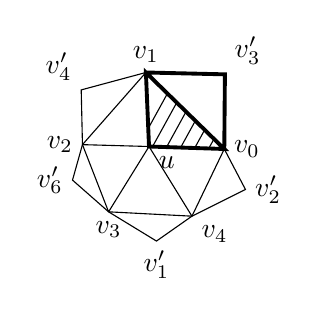
\begin{tikzpicture}[scale=.79]
\coordinate (u) at (0,0);\coordinate (a) at (1.21,-.04);\coordinate (b) at (-.05,1.19);\coordinate (c) at (-1.07,.03);\coordinate (d) at (-.65,-1.05);\coordinate (e) at (.69,-1.12);
\coordinate (aa) at (-1.23,-.54);\coordinate (bb) at (.12,-1.52);\coordinate (cc) at (1.55,-.69);\coordinate (dd) at (1.22,1.16);\coordinate (ee) at (-1.09,.91);
\draw (a)--(b)--(c)--(d)--(e)--cycle (u)--(c) (u)--(d) (u)--(e);
\draw (c)--(aa)--(d) (d)--(bb)--(e) (e)--(cc)--(a) (c)--(ee)--(b);
\draw[line width=1.4pt] (u)--(b)--(a)--cycle (b)--(dd)--(a);
\begin{scope}\clip (u)--(b)--(a)--cycle;\foreach \x in {-.2,.03,.26,.49,.72,.95}{\draw[thin] (\x,-.05)--++(.55,1);}\end{scope}
\node[below right] at(u){$u$};\node[right] at(a){$v_0$};\node[above] at(b){$v_1$};\node[left] at(c){$v_2$};\node[below] at(d){$v_3$};\node[below right] at(e){$v_4$};
\node[left] at(aa){$v'_{6}$};\node[below] at(bb){$v'_1$};\node[right] at(cc){$v'_2$};\node[above right] at(dd){$v'_3$};\node[above left] at(ee){$v'_4$};
\end{tikzpicture}}

$(u,v,w)$ forment un triangle,

\[
\det(u+v+w)=\underbrace{\det u+\det v+\det w}_{3\alpha=\alpha}
+\underbrace{\varphi(u,v)+\varphi(v,w)+\varphi(w,u)}_{\deleted{\unsure{\alpha'}}\quad3\alpha'=\alpha'}=1
\]

% archive sheet number: 15
